\documentclass[acmart, nonacm]{acmart}

\let\Bbbk\relax

%\usepackage{mathpazo}
\usepackage{url}
%\usepackage{xspace}
\usepackage{listings}
\usepackage{amsmath}
\usepackage{amssymb}
\usepackage{amsthm}
\usepackage{hyperref}
\usepackage{lipsum}
\usepackage{graphicx}
\usepackage{datetime}
\usepackage{xspace}
\usepackage{proof}
\usepackage{xcolor}
\usepackage{listings}
\usepackage{geometry}
\usepackage{float}

\usepackage{natbib}

\usepackage{fancyhdr}
\usepackage{cleveref}
\usepackage[T1]{fontenc}
\usepackage{palatino}
\usepackage{fancyvrb}


\pagestyle{fancy}
\renewcommand{\sectionmark}[1]{\markright{\textsc{#1}}}
\fancyhf{}
\rhead{\thepage }
\lhead{\rightmark }
\lfoot{{\sc Lecture Notes}}
\rfoot{ \mydate }

\begin{document}

\makeatletter
\let\@authorsaddresses\@empty
\makeatother

\title{\textsc{IADI Project Report}}
\author{Daniel Eugénio 59797}
\email{d.eugenio@campus.fct.unl.pt}
\author{Francisco Costa 60220}
\email{fd.costa@campus.fct.unl.pt}
\author{Rafael Costa 60441}
\email{rms.costa@campus.fct.unl.pt}
\newcommand{\mydate}{}
\date{\mydate}

\maketitle

\tableofcontents

\newpage
%-------------------System Architecture-------------------------
\section{System Architecture}

Our system architecture is centered around a microservices design, emphasizing the interactions and seamless communication between these services.
\begin{figure}[h]
    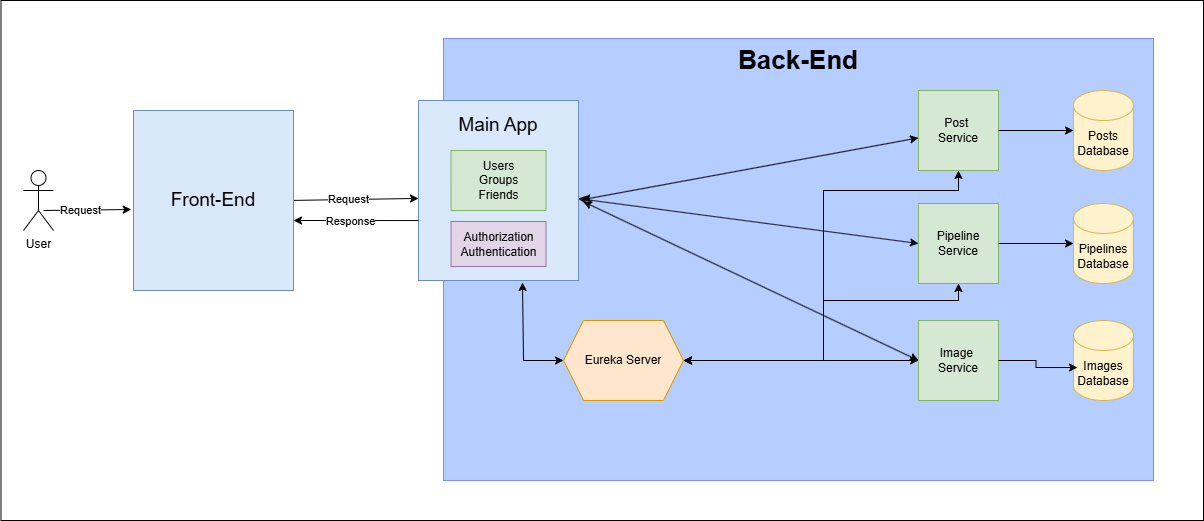
\includegraphics[width=\textwidth]{../Microservice Architecture/SystemDiagram}
    \caption{System Diagram}
\end{figure}

%-------------------User Stories-------------------------
\section{User Stories}
\textbf{Completed} User Stories:
\begin{enumerate}
    \item As an unregistered user, I want to access the picastlo social network homepage to see the first page of the public timeline of the system.
    \item As an unregistered user, I want to access the picastlo social network homepage to see a page of the public timeline of the system to see another page of public timeline of 
    the system (next, previous, any number in between).
    \item As an unregistered user, I want to access the picastlo social network homepage to sign in to the system and see the homepage of the system.
    \item As a registered user, I want to access the picastlo social network homepage to see the homepage and see the first page of my own timeline with my posts, the public posts, my friends 
    post, and the posts of the groups I am registered in.
    \item As a registered user, I want to access the picastlo social network homepage to see a page of my own timeline to see another page of my own timeline of the system 
    (next, previous, any number in between).
    \item As a registered user, I want to access the picastlo social network homepage and select my profile to see my own posts and my own pipelines.
    \item As a registered user, I want to access the picastlo social network homepage and select a group that I am registered in to see the first page of the posts in that timeline.
    \item As a registered user, I want to access the picastlo social network homepage and select a page of the timeline of a group that I am registered in to see another page of the posts in that timeline
    (next, previous, any number in between).
    \item As a user, I want to access the picastlo social network homepage to see the first page of the list of users of the system.
    \item As a user, I want to access a page of the list of users of the system to see another page of the list of users of the system (next, previous, any number in between).
    \item As a user, I want to search the list of users by username and name.
    \item As a user, I want to select a user from the list of users and see their profile.
    \item As a user, I want to use the picastlo GUI to produce an image and export it.
    \item As a user, I want to select a pipeline from the user profile and load it in picastlo GUI.
    \item As a user, I want to exit the picastlo GUI and return to the homepage of the social network.
    \item As a user, I want to select a pipeline from a post and load it in picastlo GUI.
    \item As a registered user, I want to save a picastlo pipeline from the picastlo GUI to my profile.
\end{enumerate}

%-------------------Application and Microservices-------------------------
\section{Application and Microservices}
The application is structured into a primary core application and three distinct microservices: \textbf{Images}, \textbf{Posts} and \textbf{Pipelines}.
In the core application there are three resources: \textbf{Users}, \textbf{Groups} and \textbf{Friends}.

%-------------------Users-------------------------
\subsection{Users}
The Users API provides functionality for user authentication and management. It includes endpoints for login, user creation and two user search options: retrieving all users or fetching a 
specific user by their username.
\begin{itemize}
    \item \textbf{Create User} (POST /users) - Requires username and password and returns 200 if the user was created sucessfully.
    \item \textbf{Login} (POST /users/login) - Requires username and password and returns 200 if the user was created sucessfully.
    \item \textbf{Get All Users} (GET /users) - Returns a list of all usernames.
    \item \textbf{Get a User} (GET /users/{username}) - Requires an username and returns the user if any user exists with such username.
\end{itemize}

%-------------------Groups-------------------------
\subsection{Groups}
The Groups API offers functionality to create groups, add members to a group and retrieve group information in three ways: obtaining full details of a group, listing the members of a group 
and fetching all groups associated with a specific user.
\begin{itemize}
    \item \textbf{Create Group} (POST /groups) - Requires a name and the username and returns 200 if the group was created sucessfully.
    \item \textbf{Add User To Group} (PUT /groups/{id}/{username}) - Requires the group ID and the username of the user to be added and returns the updated group information.
    \item \textbf{Get All User's Groups} (GET /groups/mygroups) - Returns a list of all groups that the logged-in user is a member of.
    \item \textbf{Get a Group} (GET /groups/{id}) - Requires an id and returns the group information if any group exists with such id.
    \item \textbf{Get a Group Members} (GET /groups/{id}/members) - Requires an id and returns the members of the group if any group exists with such id.
\end{itemize}

%-------------------Friends-------------------------
\subsection{Friends}
The Friends API provides friends management and a way to get the friend list of a user.
\begin{itemize}
    \item \textbf{Add a New Friend} (POST /friends/{username}) - Requires a username and returns 200 if the user exists and was added to the friend list.
    \item \textbf{Remove a Friend} (DELETE /friends/{username}) - Requires a username and returns 200 if the user exists and was removed from the friend list.
    \item \textbf{Get a User's Friends} (GET /friends) - Returns a list of the friends of the logged-in user.
\end{itemize}

%-------------------Posts-------------------------
\subsection{Posts}
The Posts API allows for comprehensive post management, including publishing, updating, and deleting posts. It also provides multiple retrieval options: fetching a post by its ID, 
all public posts, all personal posts, all posts within a specific group, or an individual user's feed.
\begin{itemize}
    \item \textbf{Publish a Post} (POST /post) - Requires a username, a image id, an optional pipeline id and a description and returns 200 if the post was created sucessfully.
    \item \textbf{Remove a Post} (DELETE /post/{id}) - Requires a post id and the updated information and returns the updated post information if it was sucessful.
    \item \textbf{Update a Post} (PUT /post/{id}) - Requires a post id and returns 200 if the post was deleted sucessfully.
    \item \textbf{Get a Post} (GET /post/{id}) - Requires a post id and returns the post if any post exists with such id.
    \item \textbf{Get Public Posts} (GET /post/public) - Returns a list of posts with Public visibility.
    \item \textbf{Get Personal Posts} (GET /post/personal) - Returns a list of the logged-in user's posts.
    \item \textbf{Get a Group Posts} (GET /post/group/{id}) - Requires a group id and returns a list of its' posts.
    \item \textbf{Get an User Feed} (GET /post/feed) - Returns the logged-in user's feed, which is a combination of public posts, friends' posts, and group posts.
\end{itemize}

For security, it was created five rules to produce capabilities:
\begin{enumerate}
    \item \textbf{canUpdateOrDeletePost} (@PreAuthorize) - Makes sure that only the owner of the post can update or delete the given post.
    \item \textbf{canPublish} (@PreAuthorize) - Makes sure that the post can be published with the given id.
    \item \textbf{canViewPost} (@PreAuthorize) - Verifies whether the user has the necessary permissions to view the specified post.
    \item \textbf{canViewMyPosts} \& \textbf{canViewMultiplePosts} (@PostFilter) - Verifies whether the user can in fact view the given posts and only returns the ones that the user has 
    access to.
\end{enumerate}

%-------------------Pipelines-------------------------
\subsection{Pipelines}
The Pipelines API allows for pipeline management, including creating and updating its visibility. It also provides multiple retrieval options: getting a pipeline by its ID, a public pipeline 
by its ID and all pipelines of a specific user.
\begin{itemize}
    \item \textbf{Create Pipeline} (POST /pipeline) - Requires a name and the username and returns 200 if the group was created sucessfully.
    \item \textbf{Update Pipeline Visibility} (PUT /pipeline/{id}) - Requires the pipeline ID and the updated visibility and returns the updated pipeline information.
    \item \textbf{Get All User's Pipelines} (GET /pipeline/all/{username}) - Requires an username and returns a list of all pipelines that the user has saved in its profile.
    \item \textbf{Get a Pipeline} (GET /pipeline/{id}) - Requires an id and returns the pipeline information, provided that a pipeline with the specified ID exists and the user has the 
    necessary permissions to access it.
    \item \textbf{Get a Public Pipeline} (GET /pipeline/public/{id}) - Requires an id and returns the public pipeline information if any pipeline exists with such id.
\end{itemize}

For security, it was created three rules to produce capabilities:
\begin{enumerate}
    \item \textbf{canUpdatePipeline} (@PreAuthorize) - Makes sure that only the owner of the pipeline can update the given pipeline.
    \item \textbf{canReadPipeline} (@PreAuthorize) - Verifies whether the user has the necessary permissions to view the specified pipeline.
    \item \textbf{canReadMultiplePipelines} (@PostFilter) - Verifies whether the user can in fact view the given pipelines and only returns the ones that the user has access to.
\end{enumerate}

%-------------------Images-------------------------
\subsection{Images}
The Images API provides functionality for creating and deleting images, as well as retrieval options: fetching an image by its ID or all images posted by a specific user.
\begin{itemize}
    \item \textbf{Create Image} (POST /images) - Requires a name and the username and returns 200 if the group was created sucessfully.
    \item \textbf{Delete Image} (PUT /images/{id}) - Requires the pipeline ID and the updated visibility and returns the updated pipeline information.
    \item \textbf{Get All User's Images} (GET /images/user/{username}) - Requires an username and returns a list of all images that the user has saved in its profile.
    \item \textbf{Get a Image} (GET /images/{id}) - Requires an id and returns the image information, provided that a image with the specified ID exists and the user has the 
    necessary permissions to access it.
    \item \textbf{Get a Public Image} (GET /images/public/{id}) - Requires an id and returns the public image information if any image exists with such id.
\end{itemize}

For security, it was created three rules to produce capabilities:
\begin{enumerate}
    \item \textbf{canUpdateOrDeleteImage} (@PreAuthorize) - Makes sure that only the owner of the image can update or delete the given image.
    \item \textbf{canReadImage} (@PreAuthorize) - Verifies whether the user has the necessary permissions to view the specified image.
    \item \textbf{canReadMultipleImages} (@PostFilter) - Verifies whether the user can in fact view the given images and only returns the ones that the user has access to.
\end{enumerate}

\subsection{IFML Diagram}
\begin{figure}[h]
    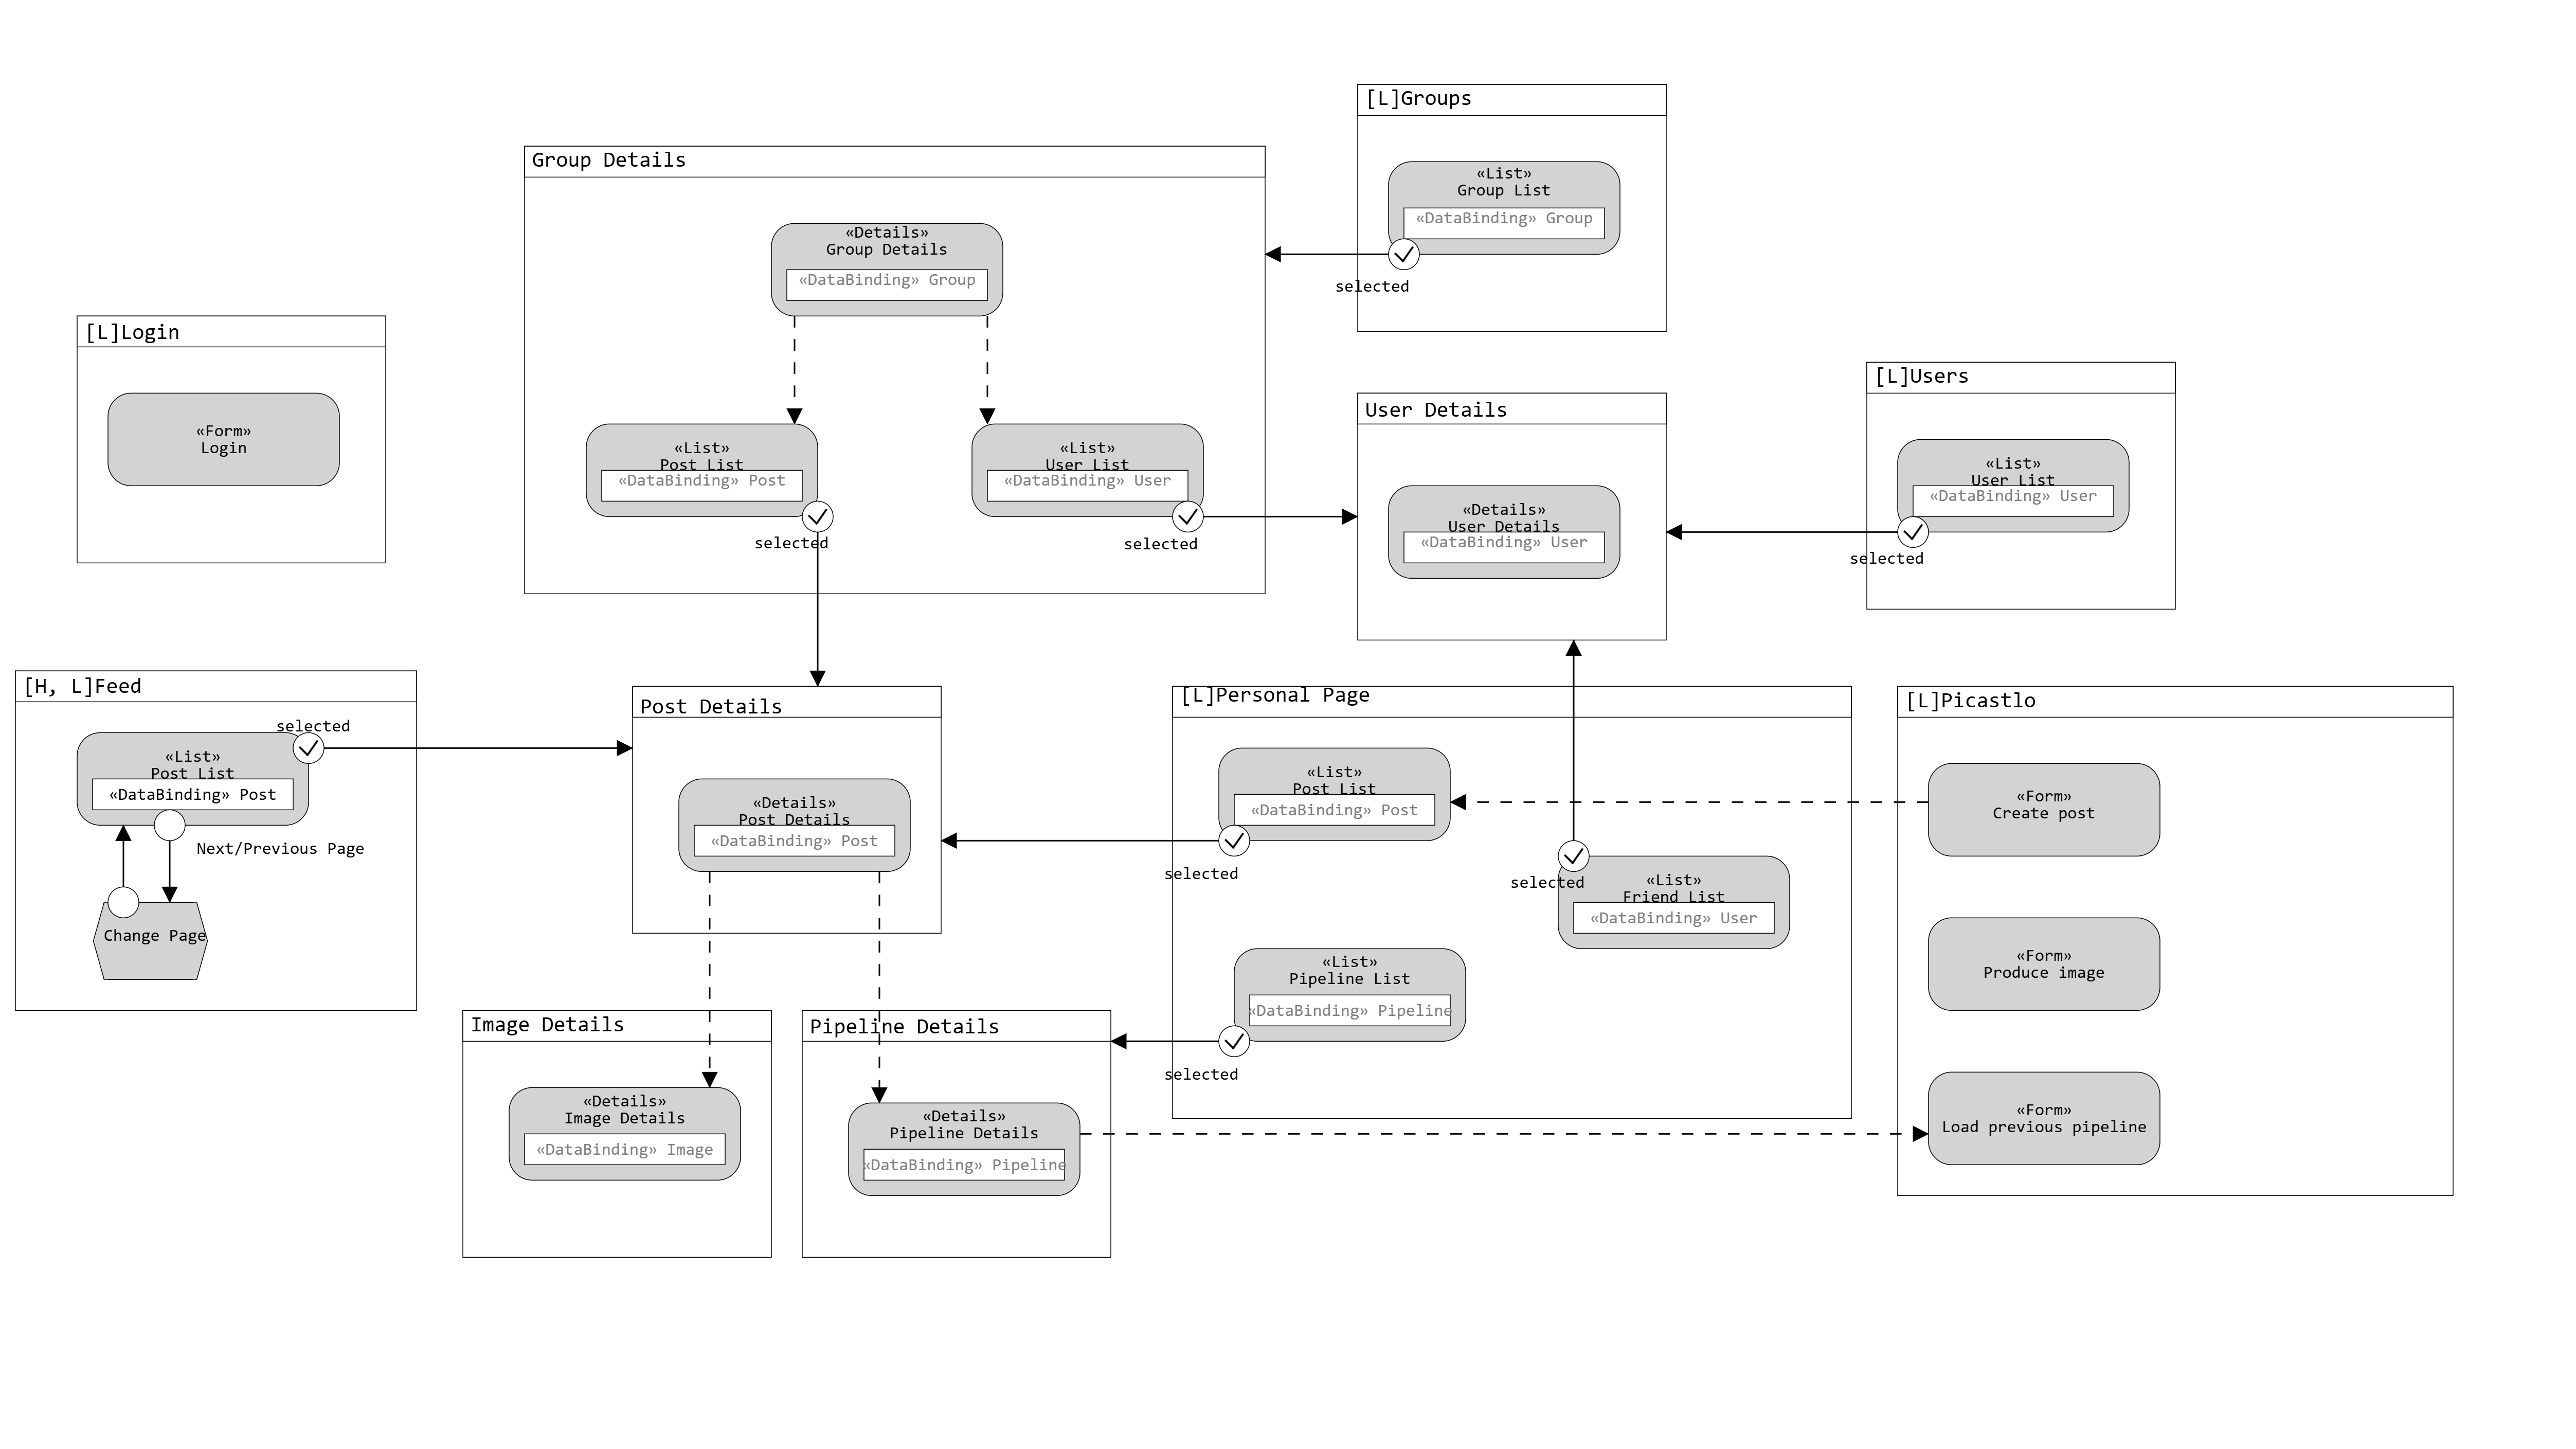
\includegraphics[width=\textwidth]{../IFML Diagram/IFMLDiagram}
    \caption{IFML Diagram}
\end{figure}


%-------------------Demo UI-------------------------
\section{Demo UI}
Link will available soon

%-------------------Assessement-------------------------
\section{Assessement}

    \begin{table}[ht]
    \centering
    \begin{tabular}{|l|c|}
    \hline
    \textbf{Topic} & \textbf{Fulfillment} \\
    \hline
    System Architecture (Micro-services) & 90\% \\
    Internal Architecture of Components (Layered Architecture, DAO, DTO, internal Services) & 95\% \\
    Architecture of Client Application (React/Redux/Async/OpenAPI) & 95\% \\
    REST API of Application & 100\% \\
    REST API of Services & 100\% \\
    Use of OpenAPI & 100\% \\
    Seed Data Used & 75\% \\
    Secure Connection between Application and Services & 85\% \\
    Completeness of Tests & 95\% \\
    Tests of security policies & >50\% \\
    \hline
    \end{tabular}
    \end{table}

%-------------------Use of AI tools-------------------------
\section{Use of Third Party Tools}
In the development of the project, we used ChatGPT as a helping tool but it was never relied upon to fully make any component since it was mainly used to fix bugs.
It was extremely helpful in identifying and fixing bugs that we were unable to detect, but there were times when even AI couldn't assist in resolving certain issues.
We also used React Material UI to help us build our front end, leveraging its available components to streamline development and ensure a consistent, modern user interface.

%-------------------Conclusion-------------------------
\section{Conclusion}
This project provided valuable insights into building a complete application and adopting the best practices to use throughout the development process. However, it wasn’t without its challenges. 
In the beginning, we faced difficulties in understanding the concept of microservices, their interactions with each other. As for the front-end part, we struggled with integrating the Picastlo 
GUI with our own website.

On the positive side, the project allowed us to deepen our knowledge of security in code and explore how separate components can seamlessly integrate to form a cohesive system.
On the other hand, a significant drawback was the time consumption of the project which took us around 350 hours in total. Developing a good application required substantial effort, which was challenging to balance alongside other 
academic commitments.

\end{document}